\documentclass[10pt]{beamer}

\usetheme{tufi}
\usepackage{wasysym}
\usepackage{ucs}
\usepackage[ngerman]{babel}
\usepackage[latin1]{inputenc}
\usepackage{amsmath,amsfonts,amssymb}
\usepackage{graphicx}
\usepackage[T1]{fontenc}
\usepackage{verbatim}
\usepackage[babel,german=quotes]{csquotes}

\usepackage{xcolor}
\usepackage{graphicx}
\usepackage[export]{adjustbox}
\usepackage{mathtools}

\def\Plus{\texttt{+}}
\def\Minus{\texttt{-}}

\makeatletter
\newcommand{\vo}{\vec{o}\@ifnextchar{^}{\,}{}}
\makeatother

\makeatletter
\newcommand{\Spvek}[2][r]{%
  \gdef\@VORNE{1}
  \left(\hskip-\arraycolsep%
    \begin{array}{#1}\vekSp@lten{#2}\end{array}%
  \hskip-\arraycolsep\right)}

\def\vekSp@lten#1{\xvekSp@lten#1;vekL@stLine;}
\def\vekL@stLine{vekL@stLine}
\def\xvekSp@lten#1;{\def\temp{#1}%
  \ifx\temp\vekL@stLine
  \else
    \ifnum\@VORNE=1\gdef\@VORNE{0}
    \else\@arraycr\fi%
    #1%
    \expandafter\xvekSp@lten
  \fi}
\makeatother

\pdfinfo
{
/Title       (Bilderkennung mit Vgg)
/Creator     (TeX)
/Author      (Justin Schartner)
}

\title{Proseminar \enquote{Convolutional Neural Networks - Methoden und Anwendungen}}
\subtitle{Bilderkennung mit Vgg}
\author{Justin Schartner}
\date{\today}

\begin{document}

\frame{\titlepage}

\AtBeginSection[]
{
\frame<handout:0>
{
\frametitle{Struktur}
\tableofcontents[currentsection,hideallsubsections]
}
}

\AtBeginSubsection[]
{
\frame<handout:0>
{
\frametitle{Struktur}
\tableofcontents[sectionstyle=show/hide,subsectionstyle=show/shaded/hide]
}
}

\newcommand<>{\highlighton}[1]{
\alt#2{\structure{#1}}{{#1}}
}

\newcommand{\icon}[1]{\pgfimage[height=1em]{#1}}

%INHALT=============================================================================
%=========================================
\section{Einleitung}
\begin{frame}
\frametitle{Thema}
\begin{block}{Problemstellung}Gibt es CNN-Architekturen, welche Bilder noch besser, als schon bekannte Architekturen klassifizieren k\"onnen?
\end{block}
\begin{block}{L\"osung}Durch die Erh\"ohung der Tiefe eines CNN verspricht man sich genauere Aussagen \"uber Bilder machen zu k\"onnen.
\end{block}
\begin{block}{Ergebnis}Die VGG-Architektur hat bewiesen, dass die Tiefe eines CNN, eine ausschlaggebende Komponente hinsichtlich der Bilder-Klassifizierung ist.
\end{block}
\end{frame}

\begin{frame}
\frametitle{Gliederung}
\begin{itemize}
	\setlength\itemsep{1em}
	\item Was ist VGG? \textbf{Allgemeines}
	\item Wie funktioniert VGG, was macht es besonders? \textbf{Architektur}
	\item Wie trainiert man ein VGG-net, was ist wichtig? \textbf{Training}
	\item Wie implementiert man ein VGG-net? \textbf{Beispiel}
	\item Wie gut ist VGG? \textbf{Bewertung}
\end{itemize}
\end{frame}
%=========================================
\section{Allgemeines}
\begin{frame}
\frametitle{Eckdaten}
\begin{itemize}
	\setlength\itemsep{1em}
	\item \textbf{V}isual \textbf{G}eometry \textbf{G}roup
	\item Department of Engineering Sciecne, University of Oxford
	\item Karen Simonyan und Andrew Zisserman
	\item \textbf{Ver\"offentlicht}: 4 Sep 2014
	\item \textbf{Letzte \"Anderung}: 10 Apr 2015
\end{itemize}
\end{frame}

\begin{frame}
\frametitle{Idee}
\begin{block}{Steigerung der Genauigkeit durch:}
\begin{itemize}
	\setlength\itemsep{1em}
	\item Steigerung der Tiefe, des CNNs
	\item Schachtelung von Convolutional-Layer-Bl\"ocken
	\item Einsatz von kleinen 3x3-Filtern und einer Stride von 1
\end{itemize}
\end{block}
\end{frame}

\begin{frame}
\frametitle{Aufgaben/ Einsatz}
\begin{block}{Bilderkennung}
\begin{itemize}
	\setlength\itemsep{1em}
	\item Imagenet
	\item Pneumoina Image
	\item Deep Facial Emotion Recognition
	\item Plankton Classification
	\item Plant Image Classification
	\item ...
\end{itemize}
\end{block}
\end{frame}

%=========================================
\section{Architektur}		
\begin{frame}
\frametitle{Architekturarten}
\begin{center}
{\tiny
\begin{tabular}{| c | c | c | c | c | c |}
\hline
\multicolumn{6}{|c|}{ConvNet Configuration} \\
\hline
A & A-LRN & B & C & D & E \\
\hline
\vtop{\hbox{\strut 11 weight}\hbox{\strut layers}} &
\vtop{\hbox{\strut 11 weight}\hbox{\strut layers}} &
\vtop{\hbox{\strut 13 weight}\hbox{\strut layers}} &
\vtop{\hbox{\strut 16 weight}\hbox{\strut layers}} &
\vtop{\hbox{\strut 16 weight}\hbox{\strut layers}} &
\vtop{\hbox{\strut 19 weight}\hbox{\strut layers}} \\
\hline \hline
\multicolumn{6}{|c|}{input (224 x 224 RGB-image)} \\
\hline
\vtop{\hbox{\strut conv3-64}} &
\vtop{\hbox{\strut conv3-64}\hbox{\strut \textbf{LRN}}} &
\vtop{\hbox{\strut conv3-64}\hbox{\strut \textbf{conv3-64}}} &
\vtop{\hbox{\strut conv3-64}\hbox{\strut conv3-64}} &
\vtop{\hbox{\strut conv3-64}\hbox{\strut conv3-64}} &
\vtop{\hbox{\strut conv3-64}\hbox{\strut conv3-64}} \\
\hline
\multicolumn{6}{|c|}{maxpool} \\
\hline
\vtop{\hbox{\strut conv3-128}} &
\vtop{\hbox{\strut conv3-128}} &
\vtop{\hbox{\strut conv3-128}\hbox{\strut \textbf{conv3-128}}} &
\vtop{\hbox{\strut conv3-128}\hbox{\strut conv3-128}} &
\vtop{\hbox{\strut conv3-128}\hbox{\strut conv3-128}} &
\vtop{\hbox{\strut conv3-128}\hbox{\strut conv3-128}} \\
\hline
\multicolumn{6}{|c|}{maxpool} \\
\hline
\vtop{\hbox{\strut conv3-256}\hbox{\strut conv3-256}} &
\vtop{\hbox{\strut conv3-256}\hbox{\strut conv3-256}} &
\vtop{\hbox{\strut conv3-256}\hbox{\strut conv3-256}} &
\vtop{\hbox{\strut conv3-256}\hbox{\strut conv3-256}\hbox{\strut \textbf{conv1-256}}} &
\vtop{\hbox{\strut conv3-256}\hbox{\strut conv3-256}\hbox{\strut \textbf{conv3-256}}} &
\vtop{\hbox{\strut conv3-256}\hbox{\strut conv3-256}\hbox{\strut conv3-256}\hbox{\strut \textbf{conv3-256}}} \\
\hline
\multicolumn{6}{|c|}{maxpool} \\
\hline
\vtop{\hbox{\strut conv3-512}\hbox{\strut conv3-512}} &
\vtop{\hbox{\strut conv3-512}\hbox{\strut conv3-512}} &
\vtop{\hbox{\strut conv3-512}\hbox{\strut conv3-512}} &
\vtop{\hbox{\strut conv3-512}\hbox{\strut conv3-512}\hbox{\strut \textbf{conv1-512}}} &
\vtop{\hbox{\strut conv3-512}\hbox{\strut conv3-512}\hbox{\strut \textbf{conv3-512}}} &
\vtop{\hbox{\strut conv3-512}\hbox{\strut conv3-512}\hbox{\strut conv3-512}\hbox{\strut \textbf{conv3-512}}} \\
\hline
\multicolumn{6}{|c|}{maxpool} \\
\hline
\vtop{\hbox{\strut conv3-512}\hbox{\strut conv3-512}} &
\vtop{\hbox{\strut conv3-512}\hbox{\strut conv3-512}} &
\vtop{\hbox{\strut conv3-512}\hbox{\strut conv3-512}} &
\vtop{\hbox{\strut conv3-512}\hbox{\strut conv3-512}\hbox{\strut \textbf{conv3-512}}} &
\vtop{\hbox{\strut conv3-512}\hbox{\strut conv3-512}\hbox{\strut \textbf{conv3-512}}} &
\vtop{\hbox{\strut conv3-512}\hbox{\strut conv3-512}\hbox{\strut conv3-512}\hbox{\strut \textbf{conv3-512}}} \\
\hline
\multicolumn{6}{|c|}{maxpool} \\
\hline
\multicolumn{6}{|c|}{FC-4096} \\
\hline
\multicolumn{6}{|c|}{FC-4096} \\
\hline
\multicolumn{6}{|c|}{FC-1000} \\
\hline
\multicolumn{6}{|c|}{soft-max} \\
\hline
\end{tabular}
}
\end{center}
\end{frame}

\begin{frame}
\frametitle{Architekur}
\begin{block}{Convolutional Layers}
\begin{itemize}
	\item receiptive field: 3x3, 1x1
	\item activation: RelU, stride: 1, padding: 1, channels: 64, 128, 512, 512
\end{itemize}
\end{block}
\begin{block}{Pooling Layer}
\begin{itemize}
	\item Max-Pool
	\item field: 2x2, stride: 2
\end{itemize}
\end{block}
\begin{block}{Fully-Connected Layers}
\begin{itemize}
	\item activation: RelU
	\item channels: 4096, 4096, 1000
\end{itemize}
\end{block}
\begin{block}{Softmax Layer}
\end{block}
\end{frame}

\begin{frame}
\frametitle{Convolutional Layers}
\begin{itemize}
	\setlength\itemsep{1em}
	\item 2D - Convolution
	\item Aktivierungsfunktion: ReLU
	\item Stride: 1x1
	\item Padding: 1, 0
	\item[] $\Rightarrow$ Die Breite und H\"ohe des Inputs wird beibehalten
	\item Kernel: 3x3 oder 1x1
	\item[] $\Rightarrow$ Minimaler Kernel f\"ur den Vergleich von Links/Rechts Oben/Unten
	\item Filter Anzahl: 64, 128, 256, 512
	\item[] $\Rightarrow$ Filter lernen Muster des Inputs zu erkennen 
\end{itemize}
\end{frame}

\begin{frame}
\frametitle{Convolutional Layers}
\begin{figure}
	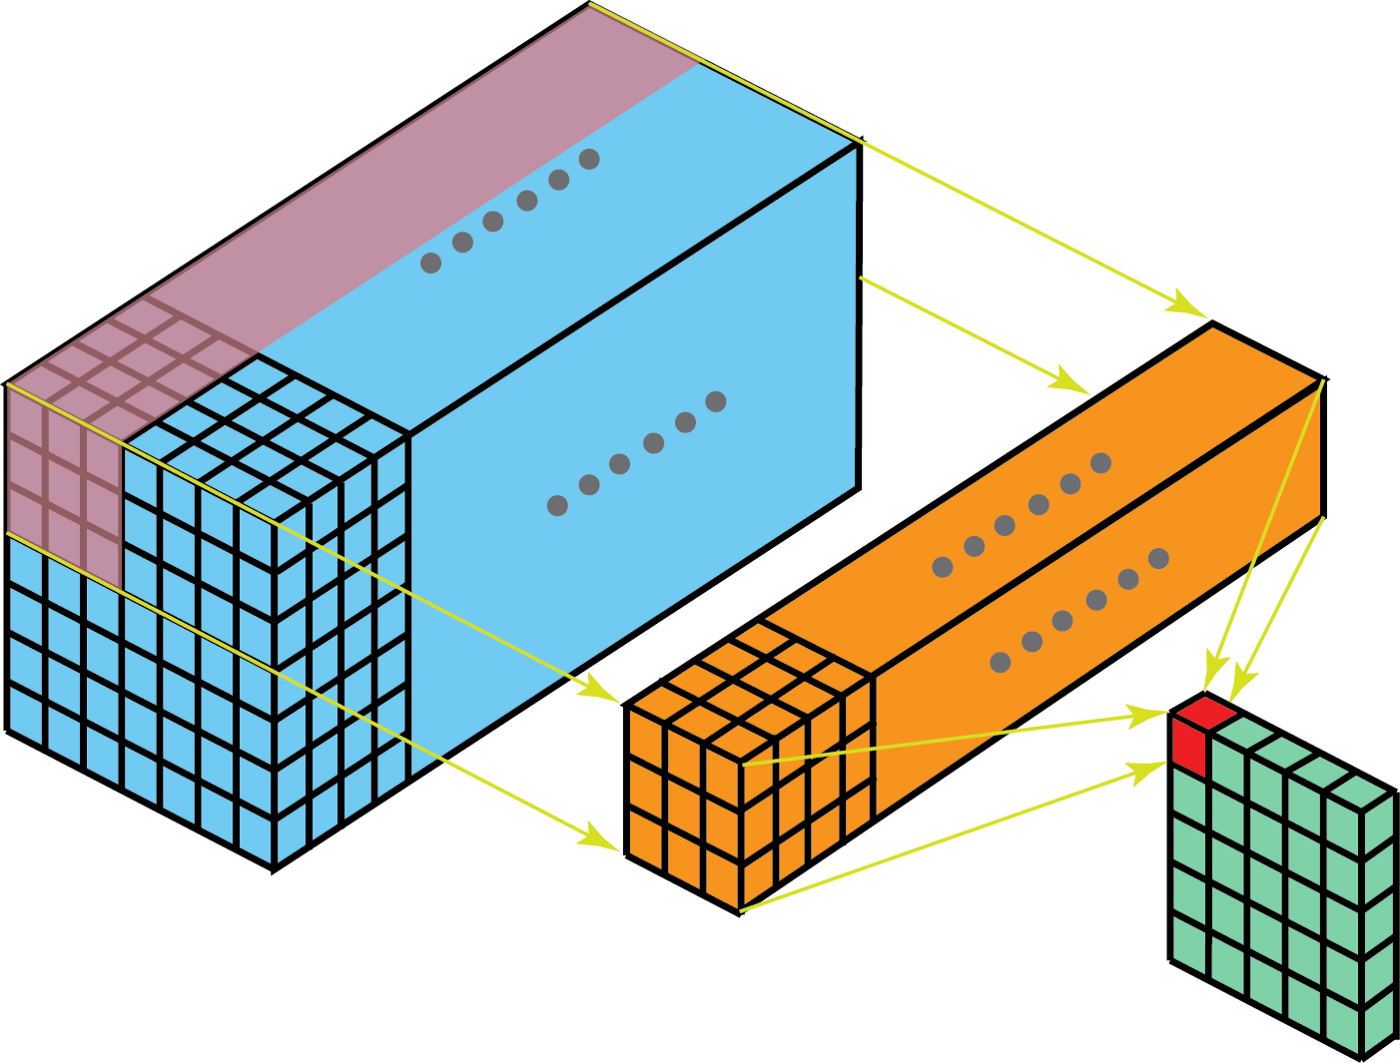
\includegraphics[width=50mm]{convolution.png}
\end{figure}
(Breite x H\"ohe x Tiefe) 
$\xrightarrow[
	\text{Conv2d(Filter: \textbf{3x3xTiefe}, Filter Anzahl: \textbf{n})}
]{}$
(Breite x H\"ohe x n)
\end{frame}

\begin{frame}
\frametitle{ReLU}
\framesubtitle{\textbf{Re}ctified \textbf{L}inerar \textbf{U}nit}
\begin{columns}
	\begin{column}{.5\textwidth}
		\begin{equation*}
				f(x) =
					\begin{cases*}
					x & x>0 \\
					0 & sonst
					\end{cases*}
		\end{equation*}\ \ \ \\
		\begin{equation*}
				f'(x) =
					\begin{cases*}
					1 & x>0 \\
					0 & x<0
					\end{cases*}
		\end{equation*}
	\end{column}

	\begin{column}{.5\textwidth}
		\begin{figure}
			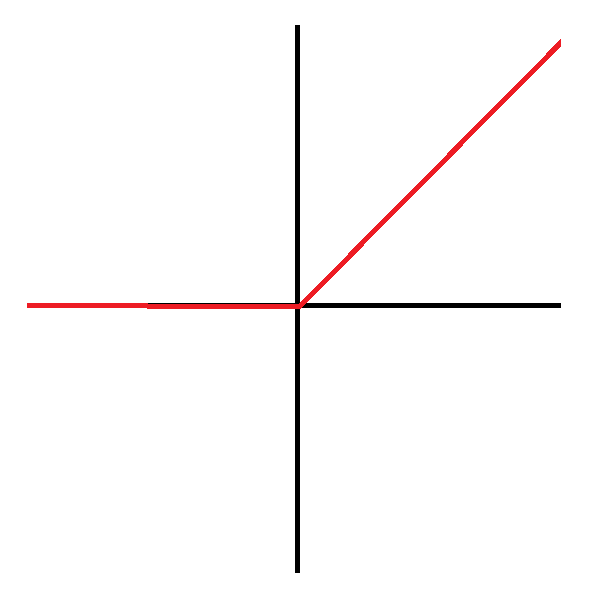
\includegraphics[width=20mm]{relu.png}
			\caption{$f(x)$}
		\end{figure}
		\begin{figure}
			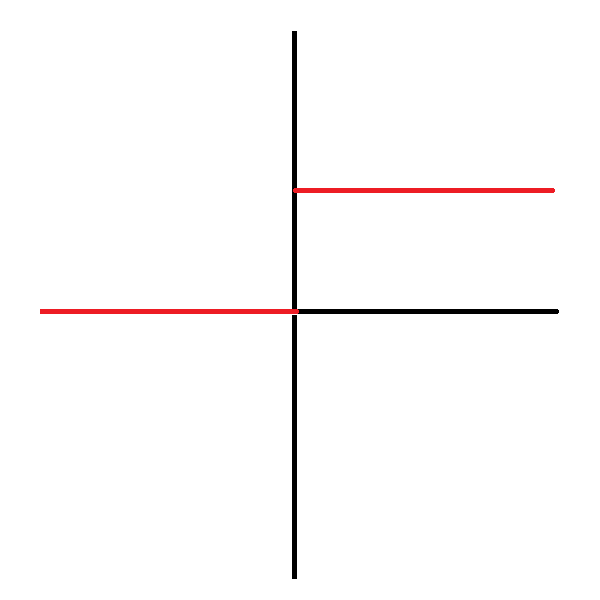
\includegraphics[width=20mm]{relu_prime.png}
			\caption{$f'(x)$}
		\end{figure}
	\end{column}
\end{columns}
\end{frame}

\begin{frame}
\frametitle{Max-Pooling}
\begin{itemize}
	\setlength\itemsep{1em}
	\item Stride: 2x2
	\item Kernel: 2x2
	\item[] $\Rightarrow$ Die Breite und H\"ohe wird halbiert
	\item[] $\Rightarrow$ Daten werden auf die auschlaggebenden Informationen reduziert
\end{itemize}
\end{frame}

\begin{frame}
\frametitle{Fully Connected Layers}
\begin{columns}
	\begin{column}{.5\textwidth}
		\begin{itemize}
			\setlength\itemsep{1em}
			\item Input: (7x7x512)
			\item[] $\Rightarrow$ (7x7x512) Input-Neuronen
			\item Aktivierungsfunktion: ReLU
			\item Zwei versteckte Layer mit jeweils 4096 Neuronen
			\item ImageNet-Klassifiezunrg von 1000 Klassen
			\item[] $\Rightarrow$ 1000 Output-Neuronen
		\end{itemize}
	\end{column}

	\begin{column}{.5\textwidth}
		\begin{figure}
			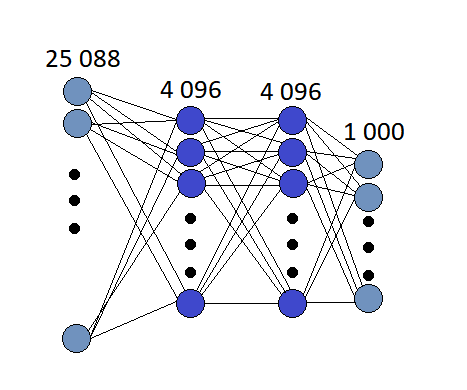
\includegraphics[width=50mm]{full_connected.png}
			\caption{full-yconnected layer}
		\end{figure}
	\end{column}

\end{columns}
\end{frame}

\begin{frame}
\frametitle{Softmax}
\begin{columns}
	\begin{column}{.5\textwidth}
		${\sigma (\vec{z})}_i = \frac{e^{z_i}}{\sum_{j=1}^{K} e^{z_j}}$ \ \\
		\begin{itemize}
			\setlength\itemsep{1em}
			\item[]
			\item normalisierte Exponentialfunktion
			\item kategoriale Verteilung
			\item Transformation in den Wertebereich [0,1]
		\end{itemize}
	\end{column}
	\begin{column}{.5\textwidth}
		\begin{figure}
			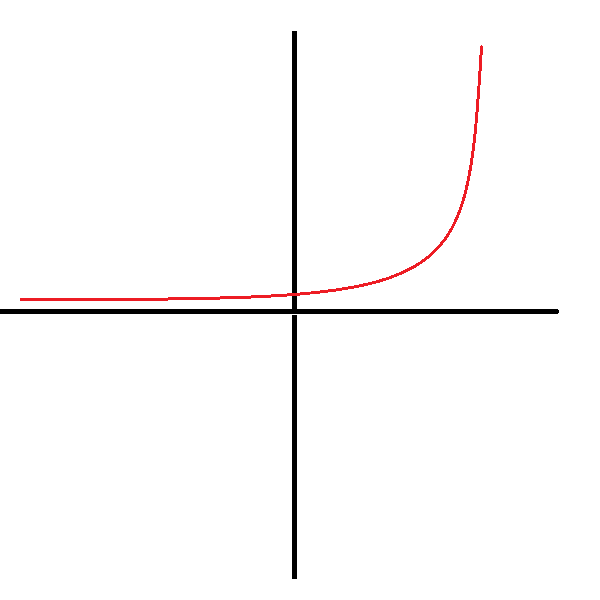
\includegraphics[width=20mm]{ehochx.png}
			\caption{$e^x$}
		\end{figure}
		\begin{align*}
			\Spvek{-0.5; 0.8; 1.3} \xRightarrow[]{Softmax} \Spvek{0.093; 0.342; 0.564} \\
		\end{align*}
	\end{column}
\end{columns}


\end{frame}

%=========================================
\section{Training}

\begin{frame}
	\frametitle{Training}
	\begin{block}{Optimierung des Traininigs durch:}
	\begin{itemize}
		\item \textbf{S}tochastic \textbf{G}radient \textbf{D}escent
		\item Dropout, p=0.5
		\item L2-Normalisation
		\item Momentum
		\item Batch-Size: 256
	\end{itemize}
	\end{block}
	\begin{block}{Weitere n\"utzliche Faktoren:}
		\begin{itemize}
			\item Kleinere Filter-Gr\"o\"sen
			\item Vor-Initialisierung von Gewichten
			\item Die Tiefe des Netzwerkes
		\end{itemize}
	\end{block}
\end{frame}

\begin{frame}
	\frametitle{Training}
	\framesubtitle{Details}
	\begin{itemize}
		\setlength\itemsep{1em}
		\item Learninig-rate: 10e-2 - 10e-4
		\item Momentum: 0.9
		\item Weight-Decay: 5e-4
		\item Biases wurden mit 0 initialisiert
		\item VGG16 wurde mit VGG11-Gewichten initialisiert
	\end{itemize}
\end{frame}

\begin{frame}
\frametitle{Training}
\framesubtitle{Bild-Processing}
\begin{itemize}
	\setlength\itemsep{1em}
	\item Bilder wurden zuf\"allig aus anderen Bildern ausgeschnitten
	\item Bilder wurden zuf\"allig horizontal gedreht
	\item Bilder wurden zuf\"allig skaliert
	\item[] $\Rightarrow$ Filter werden trainiert Features auf verschieden Arten zu erkennen 
\end{itemize}
\end{frame}

%=========================================
\section{Beispiel}

\begin{frame}
\frametitle{Vgg initialisieren}
	1. Variante: Die Komponenten einzeln erstellen und aneinander reihen.
	\begin{itemize}
		\item[] {\color{green} Anpassbarkeit an das Problem}
		\item[] {\color{red} Das Trainieren des Netzwerkes nimmt mehr Zeit in Anspruch}
 	\end{itemize}
	2. Variante: Benutzen von schon bestehenden (und trainierten) Netzwerken. 
	\begin{itemize}
		\item[] {\color{green} Sind sofort einsatzbereit}
		\item[] {\color{green} Aufwand ist kleiner}
		\item[] {\color{green} Die vortrainierten Gewichte k\"onnen die Trainingszeit minimieren}
		\item[] {\color{red} Konfigurierung kann aufwendig sein}
	\end{itemize}
\end{frame}

\begin{frame}
\frametitle{Vgg initialisieren}
\framesubtitle{1. Variante}
\begin{columns}
	\begin{column}{.5\textwidth}
		\begin{figure}
			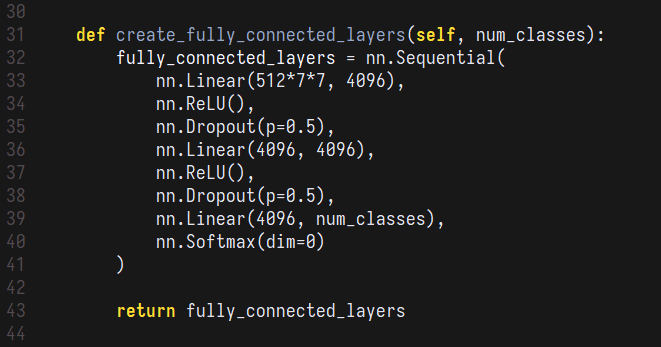
\includegraphics[width=55mm]{init_fc.png}
		\end{figure}
	\end{column}
	\begin{column}{.5\textwidth}
		\begin{figure}
			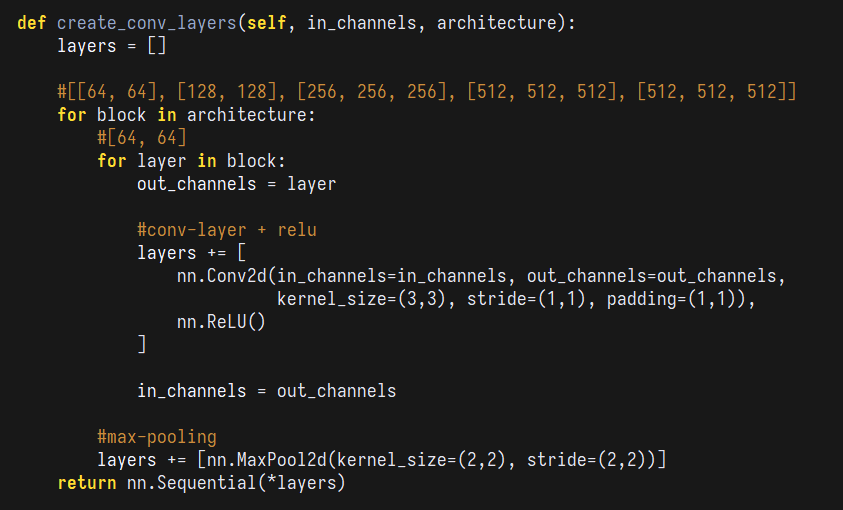
\includegraphics[width=55mm]{init_c.png}
		\end{figure}
	\end{column}
\end{columns}
\end{frame}

\begin{frame}
\frametitle{Vgg initialisieren}
\framesubtitle{1. Variante}
	\begin{figure}
		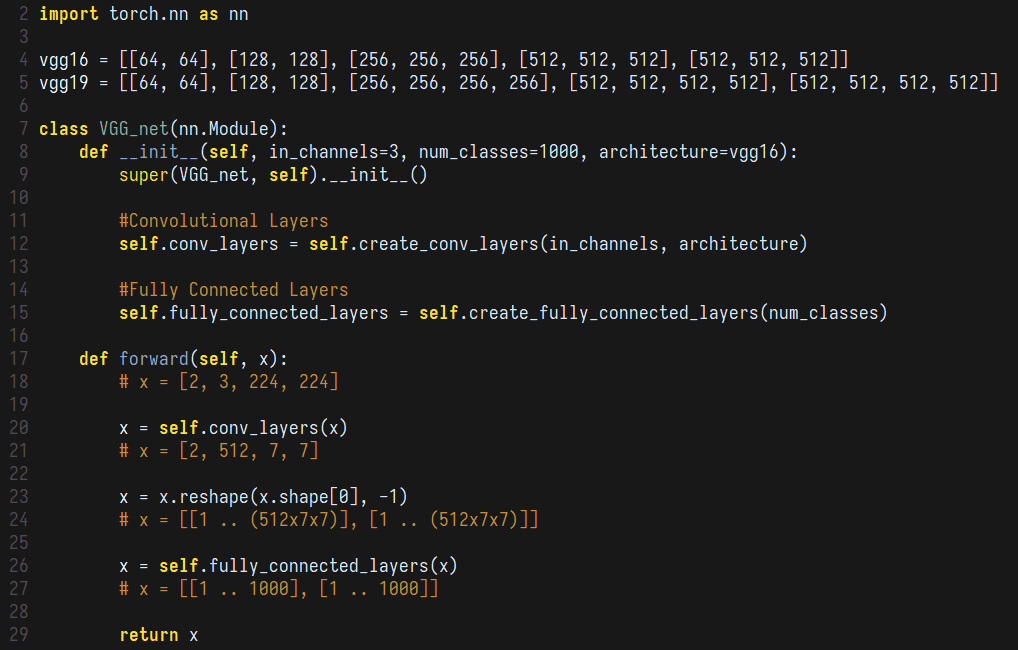
\includegraphics[width=100mm]{init_main.png}
	\end{figure}
\end{frame}

\begin{frame}
\frametitle{Vgg initialisieren}
\framesubtitle{1. Variante}
\begin{columns}
	\begin{column}{.5\textwidth}
		\begin{figure}
			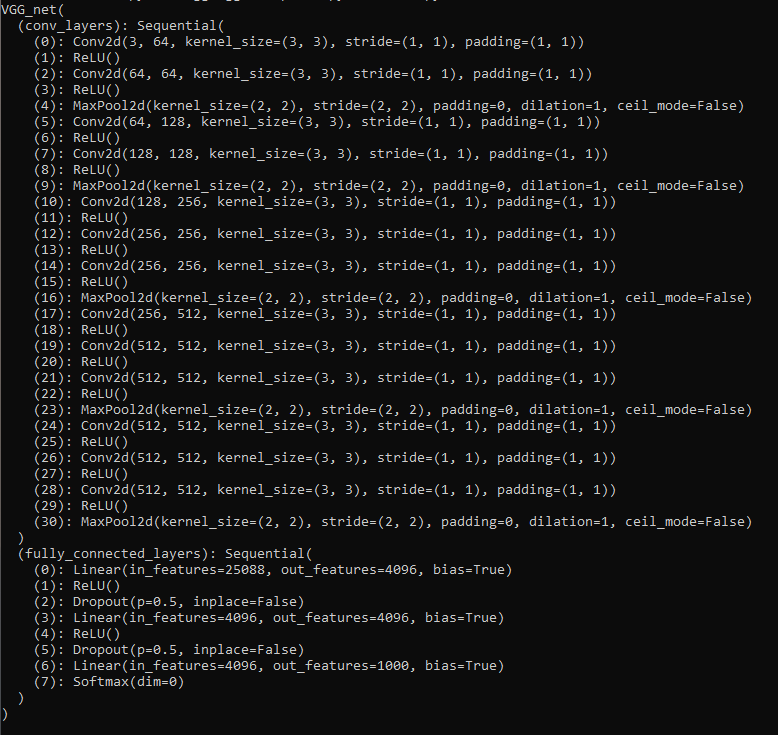
\includegraphics[width=55mm]{init_output.png}
		\end{figure}
	\end{column}
	\begin{column}{.5\textwidth}
		\begin{figure}
			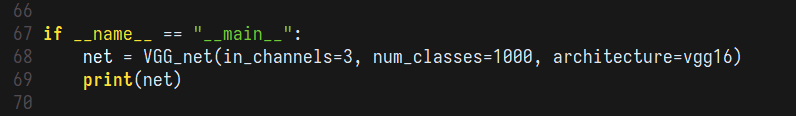
\includegraphics[width=55mm]{init_print.png}
		\end{figure}
	\end{column}
\end{columns}
\end{frame}

\begin{frame}
\frametitle{Vgg initialisieren}
\framesubtitle{2. Variante}
\begin{columns}
	\begin{column}{.5\textwidth}
		\begin{figure}
			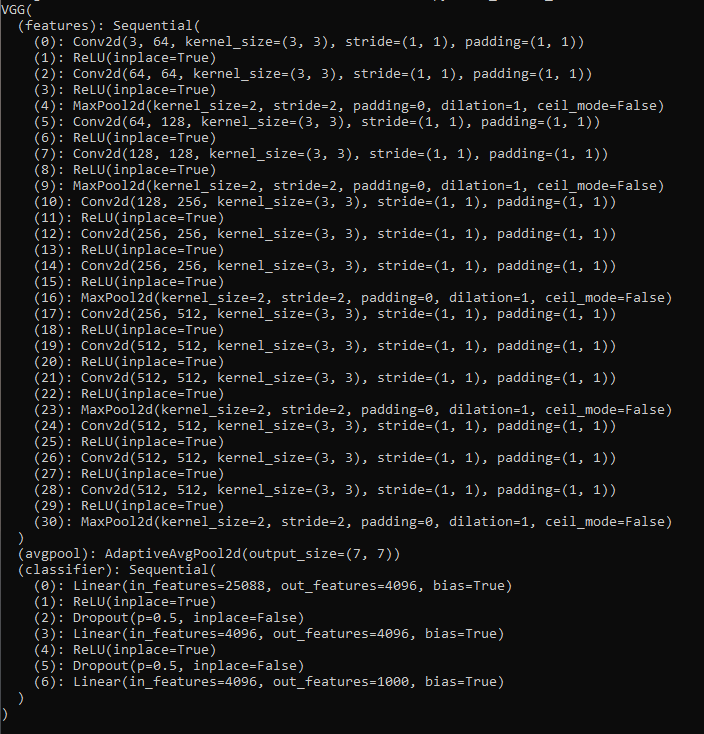
\includegraphics[width=55mm]{load_output.png}
		\end{figure}
	\end{column}
	\begin{column}{.5\textwidth}
		\begin{figure}
			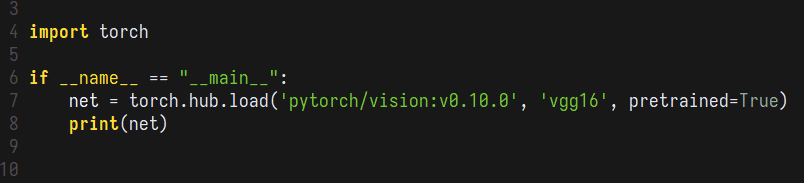
\includegraphics[width=55mm]{load.png}
		\end{figure}
	\end{column}
\end{columns}
\end{frame}

\begin{frame}
\frametitle{Vgg trainieren}
\begin{figure}
		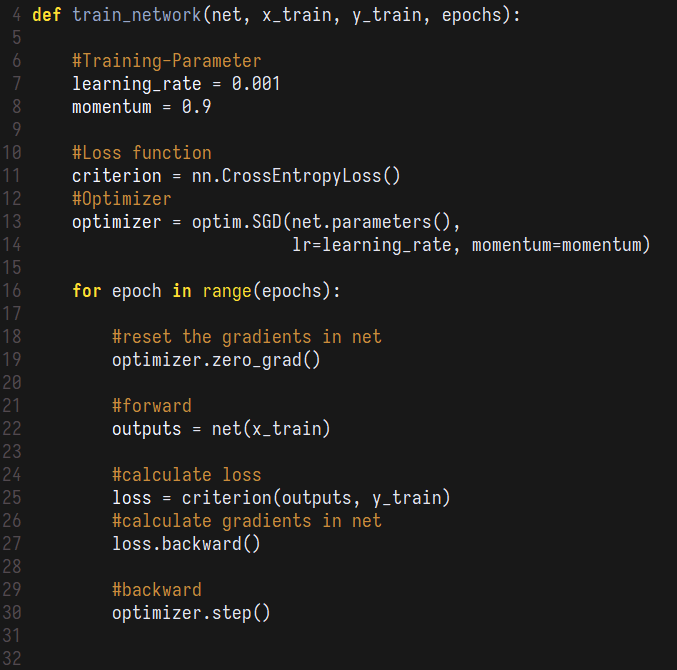
\includegraphics[width=70mm]{train.png}
	\end{figure}
\end{frame}

\begin{frame}
\frametitle{Vgg benutzen}
\begin{columns}
	\begin{column}{.5\textwidth}
		\begin{figure}
			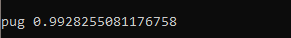
\includegraphics[width=55mm]{use_output.png}
		\end{figure}
	\end{column}
	\begin{column}{.5\textwidth}
		\begin{figure}
			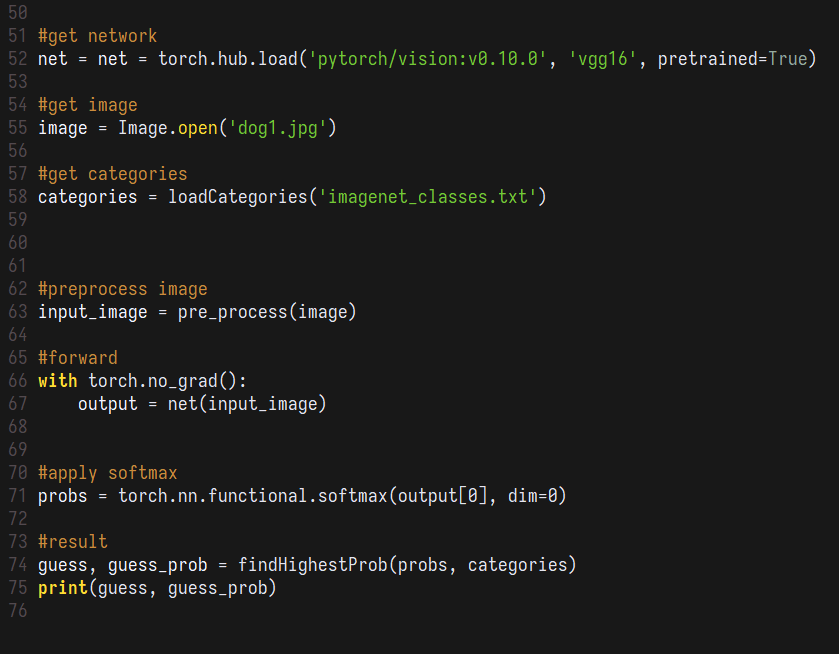
\includegraphics[width=55mm]{use.png}
		\end{figure}
	\end{column}
\end{columns}
\end{frame}

%=========================================
\section{Bewertung}

\begin{frame}
	\frametitle{Ergebnis}
	\begin{itemize}
		\item Die Anwendung von mehreren 3x3 Filtern ersetzt die Funktionalität von bsp. 7x7 Filtern und erh\"ort die Diskriminietivit\"at
		\item Die Tiefe eine CNNs ist auschlaggebend f\"ur die Genauigkeit
		\item VGG-Architekturen haben viele Anwendungsbereiche, erzielen auf verschiedensten Datenbanken erfolgreiche Resultate
	\end{itemize}
\end{frame}

\begin{frame}
	\frametitle{Komplexit\"at}
	\begin{itemize}
		\item Anzahl an Parametern: 15.1, 15.3, 20.6, 25.9 in Millionen
		\item[] $\Rightarrow$ Mehr Parameter f\"uhren zu einer l\"ängeren Trainigszeit
		\item Enspricht etwa 528MB
		\item[] $\Rightarrow$ Hoher Speicher-Verbrauch
	\end{itemize}
\end{frame}

\begin{frame}
	\frametitle{Performance}
	\begin{itemize}
		\item 2014 
	\end{itemize}
\end{frame}

\begin{frame}
	\frametitle{Vergleich}
\end{frame}

%==========================================
\section{Ausblick}
\begin{frame}
	\frametitle{Ausblick}
\end{frame}

%=========================================
\section{Quellen}
\begin{frame}
	\frametitle{Quellen}
	Kunlun Bai | A Comprehensive Introduction to Different Types of Convolutions in Deep Learning | Towards Data Science | 2022 | 18.05.2022 | (https://graphics.cs.tu-dortmund.de/fileadmin/ls7-www/seminar/2022/proseminar_cnn/material/Proseminar_CNN_SS2022_Hinweise_Praesentation.pdf) \\
\end{frame}

\end{document}